

\tikzset{every picture/.style={line width=0.75pt}} %set default line width to 0.75pt        

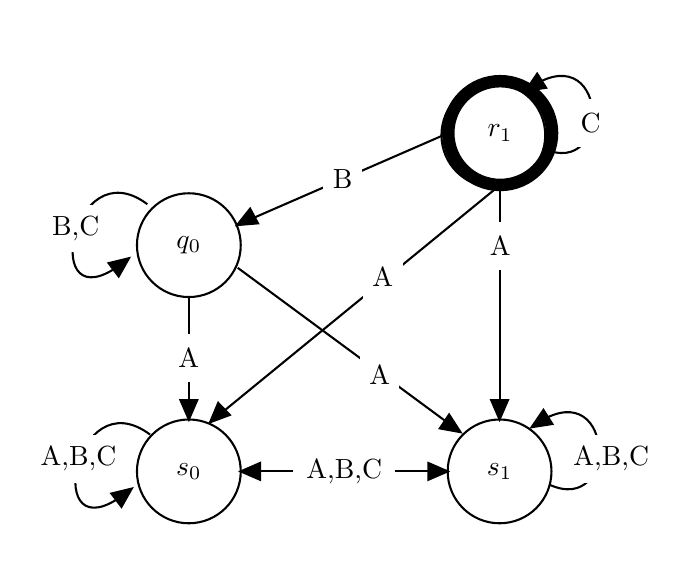
\begin{tikzpicture}[x=0.75pt,y=0.75pt,yscale=-1,xscale=1]
%uncomment if require: \path (0,300); %set diagram left start at 0, and has height of 300

%Shape: Circle [id:dp8938158972072578] 
\draw  [line width=0.75]  (135.29,223) .. controls (135.29,209.19) and (146.48,198) .. (160.29,198) .. controls (174.09,198) and (185.29,209.19) .. (185.29,223) .. controls (185.29,236.81) and (174.09,248) .. (160.29,248) .. controls (146.48,248) and (135.29,236.81) .. (135.29,223) -- cycle ;
%Shape: Circle [id:dp19780391712041556] 
\draw   (285,223) .. controls (285,209.19) and (296.19,198) .. (310,198) .. controls (323.81,198) and (335,209.19) .. (335,223) .. controls (335,236.81) and (323.81,248) .. (310,248) .. controls (296.19,248) and (285,236.81) .. (285,223) -- cycle ;
%Straight Lines [id:da018251469869151382] 
\draw    (185.29,223) -- (285,223) ;


%Shape: Triangle [id:dp4725710951486233] 
\draw  [fill={rgb, 255:red, 0; green, 0; blue, 0 }  ,fill opacity=1 ] (132.8,231.28) -- (127.82,240.08) -- (122.97,233.67) -- cycle ;
%Shape: Triangle [id:dp08394946096129607] 
\draw  [fill={rgb, 255:red, 0; green, 0; blue, 0 }  ,fill opacity=1 ] (285,223) -- (275.72,227.02) -- (275.72,218.98) -- cycle ;
%Shape: Triangle [id:dp12888926826248426] 
\draw  [fill={rgb, 255:red, 0; green, 0; blue, 0 }  ,fill opacity=1 ] (185.29,223) -- (194.56,218.98) -- (194.56,227.02) -- cycle ;
%Shape: Triangle [id:dp7536519811814515] 
\draw  [fill={rgb, 255:red, 0; green, 0; blue, 0 }  ,fill opacity=1 ] (325.43,201.72) -- (331.13,193.37) -- (335.42,200.17) -- cycle ;
%Curve Lines [id:da0862450190271058] 
\draw    (141.62,205.27) .. controls (104.82,177.67) and (89.1,264.08) .. (129.1,234.08) ;


%Curve Lines [id:da8507870813478686] 
\draw    (325.43,201.72) .. controls (365.43,171.72) and (368.63,245.32) .. (333.83,229.32) ;


%Shape: Circle [id:dp06782137726568571] 
\draw  [line width=0.75]  (135.29,114) .. controls (135.29,100.19) and (146.48,89) .. (160.29,89) .. controls (174.09,89) and (185.29,100.19) .. (185.29,114) .. controls (185.29,127.81) and (174.09,139) .. (160.29,139) .. controls (146.48,139) and (135.29,127.81) .. (135.29,114) -- cycle ;
%Shape: Triangle [id:dp8413979641210945] 
\draw  [fill={rgb, 255:red, 0; green, 0; blue, 0 }  ,fill opacity=1 ] (131.46,120.28) -- (126.49,129.08) -- (121.64,122.67) -- cycle ;
%Shape: Triangle [id:dp7368099608094223] 
\draw  [fill={rgb, 255:red, 0; green, 0; blue, 0 }  ,fill opacity=1 ] (291.18,204.1) -- (281.23,202.29) -- (285.69,195.61) -- cycle ;
%Curve Lines [id:da6315070066186073] 
\draw    (140.29,94.27) .. controls (103.49,66.67) and (87.76,153.08) .. (127.76,123.08) ;


%Straight Lines [id:da7382395640533164] 
\draw    (160.29,139) -- (160.29,198) ;


%Straight Lines [id:da3690444677581517] 
\draw    (183.87,124.94) -- (291.18,204.1) ;


%Shape: Triangle [id:dp417855807516911] 
\draw  [fill={rgb, 255:red, 0; green, 0; blue, 0 }  ,fill opacity=1 ] (160.29,198) -- (156.27,188.72) -- (164.3,188.72) -- cycle ;
%Shape: Circle [id:dp5972014220045965] 
\draw  [line width=4.5]  (285.29,60) .. controls (285.29,46.19) and (296.48,35) .. (310.29,35) .. controls (324.09,35) and (335.29,46.19) .. (335.29,60) .. controls (335.29,73.81) and (324.09,85) .. (310.29,85) .. controls (296.48,85) and (285.29,73.81) .. (285.29,60) -- cycle ;
%Shape: Triangle [id:dp4971926593318259] 
\draw  [fill={rgb, 255:red, 0; green, 0; blue, 0 }  ,fill opacity=1 ] (170.53,199.33) -- (174.44,190.01) -- (180.01,195.81) -- cycle ;
%Straight Lines [id:da46185098746714237] 
\draw    (310.29,85) -- (310.29,193.36) ;


%Straight Lines [id:da9004694794581629] 
\draw    (310.29,85) -- (170.53,199.33) ;


%Shape: Triangle [id:dp3663238051701312] 
\draw  [fill={rgb, 255:red, 0; green, 0; blue, 0 }  ,fill opacity=1 ] (310,198) -- (305.98,188.72) -- (314.02,188.72) -- cycle ;
%Shape: Circle [id:dp9462184779936802] 
\draw   (282,61) .. controls (282,47.19) and (293.19,36) .. (307,36) .. controls (320.81,36) and (332,47.19) .. (332,61) .. controls (332,74.81) and (320.81,86) .. (307,86) .. controls (293.19,86) and (282,74.81) .. (282,61) -- cycle ;
%Shape: Triangle [id:dp5745677700051097] 
\draw  [fill={rgb, 255:red, 0; green, 0; blue, 0 }  ,fill opacity=1 ] (322.43,39.72) -- (328.13,31.37) -- (332.42,38.17) -- cycle ;
%Curve Lines [id:da6922101751426857] 
\draw    (322.43,39.72) .. controls (362.43,9.72) and (365.63,83.32) .. (330.83,67.32) ;


%Straight Lines [id:da08547301161768894] 
\draw    (285.29,60) -- (183.53,104.33) ;


%Shape: Triangle [id:dp20482466216590445] 
\draw  [fill={rgb, 255:red, 0; green, 0; blue, 0 }  ,fill opacity=1 ] (183.53,104.33) -- (189.81,96.41) -- (193.6,103.49) -- cycle ;

% Text Node
\draw (160.29,223) node  [align=left] {$s_0$};
% Text Node
\draw (310,223) node  [align=left] {$s_1$};
% Text Node
\draw  [color={rgb, 255:red, 255; green, 255; blue, 255 }  ,draw opacity=1 ][fill={rgb, 255:red, 255; green, 255; blue, 255 }  ,fill opacity=1 ]  (211.14,212) -- (259.14,212) -- (259.14,234) -- (211.14,234) -- cycle  ;
\draw (235.14,223) node  [align=left] {A,B,C};
% Text Node
\draw  [color={rgb, 255:red, 255; green, 255; blue, 255 }  ,draw opacity=1 ][fill={rgb, 255:red, 255; green, 255; blue, 255 }  ,fill opacity=1 ]  (83.14,206) -- (131.14,206) -- (131.14,228) -- (83.14,228) -- cycle  ;
\draw (107.14,217) node  [align=left] {A,B,C};
% Text Node
\draw  [color={rgb, 255:red, 255; green, 255; blue, 255 }  ,draw opacity=1 ][fill={rgb, 255:red, 255; green, 255; blue, 255 }  ,fill opacity=1 ]  (339.81,206) -- (387.81,206) -- (387.81,228) -- (339.81,228) -- cycle  ;
\draw (363.81,217) node  [align=left] {A,B,C};
% Text Node
\draw (160.29,114) node  [align=left] {$q_0$};
% Text Node
\draw  [color={rgb, 255:red, 255; green, 255; blue, 255 }  ,draw opacity=1 ][fill={rgb, 255:red, 255; green, 255; blue, 255 }  ,fill opacity=1 ]  (89.31,95) -- (122.31,95) -- (122.31,117) -- (89.31,117) -- cycle  ;
\draw (105.81,106) node  [align=left] {B,C};
% Text Node
\draw  [color={rgb, 255:red, 255; green, 255; blue, 255 }  ,draw opacity=1 ][fill={rgb, 255:red, 255; green, 255; blue, 255 }  ,fill opacity=1 ]  (151.29,157.5) -- (169.29,157.5) -- (169.29,179.5) -- (151.29,179.5) -- cycle  ;
\draw (160.29,168.5) node  [align=left] {A};
% Text Node
\draw  [color={rgb, 255:red, 255; green, 255; blue, 255 }  ,draw opacity=1 ][fill={rgb, 255:red, 255; green, 255; blue, 255 }  ,fill opacity=1 ]  (243.27,165.77) -- (261.27,165.77) -- (261.27,187.77) -- (243.27,187.77) -- cycle  ;
\draw (252.27,176.77) node  [align=left] {A};
% Text Node
\draw (310.29,60) node  [align=left] {$r_1$};
% Text Node
\draw  [color={rgb, 255:red, 255; green, 255; blue, 255 }  ,draw opacity=1 ][fill={rgb, 255:red, 255; green, 255; blue, 255 }  ,fill opacity=1 ]  (301.29,103.5) -- (319.29,103.5) -- (319.29,125.5) -- (301.29,125.5) -- cycle  ;
\draw (310.29,114.5) node  [align=left] {A};
% Text Node
\draw  [color={rgb, 255:red, 255; green, 255; blue, 255 }  ,draw opacity=1 ][fill={rgb, 255:red, 255; green, 255; blue, 255 }  ,fill opacity=1 ]  (244.77,118.27) -- (262.77,118.27) -- (262.77,140.27) -- (244.77,140.27) -- cycle  ;
\draw (253.77,129.27) node  [align=left] {A};
% Text Node
\draw  [color={rgb, 255:red, 255; green, 255; blue, 255 }  ,draw opacity=1 ][fill={rgb, 255:red, 255; green, 255; blue, 255 }  ,fill opacity=1 ]  (344.31,44) -- (363.31,44) -- (363.31,66) -- (344.31,66) -- cycle  ;
\draw (353.81,55) node  [align=left] {C};
% Text Node
\draw  [color={rgb, 255:red, 255; green, 255; blue, 255 }  ,draw opacity=1 ][fill={rgb, 255:red, 255; green, 255; blue, 255 }  ,fill opacity=1 ]  (225.41,71.17) -- (243.41,71.17) -- (243.41,93.17) -- (225.41,93.17) -- cycle  ;
\draw (234.41,82.17) node  [align=left] {B};


\end{tikzpicture}
